% ============================ Enrico Ribiani 16-03-2021 ====================================================================
% -------------classe documento -------------------
\documentclass{article}
% ------------ pacchetti necessari ----------------

\usepackage{graphicx}   % need for figure
\usepackage{biblatex}   % citazioni
\usepackage{amsfonts}   % if you want the fonts
\usepackage{amssymb}    % if you want extra symbols
\usepackage{graphicx}   % need for figures
\usepackage{mathptmx}
\usepackage{float}% ---------====== MOLTO IMPORTANTE PER METTERE TABELLE E FIGURE DOVE SI VUOLE ES \begin{coso}[H]
\usepackage[utf8]{inputenc}
\usepackage{textcomp}
\usepackage[hang,flushmargin,bottom]{footmisc} % footnote format
\usepackage{fancyhdr, lastpage}
\usepackage{titlesec}
\titleformat{\section}{\normalsize\bfseries}{\thesection.}{1em}{}	% required for heading numbering style
%===================inizio pagina del titolo=================
\begin{document}
    \begin{titlepage}
		\begin{center}
% ------------------ inizio immagine logo ----------
\begin{figure}
    \centering
    
\includegraphics{logo.png}
 %   \caption{Caption}
    \label{fig:logo}
\end{figure}
% ------------------ fine immagine logo ----------
\large Enrico Ribiani\\
\large 3AUB\\
\vfill

\Huge{\textbf{Carica e scarica di un condensatore.}}\\
\vfill

\LARGE{Esperienza numero 8 }\\
\vfill
\LARGE{\textbf{Scopo:} Verificare il comportamento di un condensatore carica scarica in funzione di \textit{T}}\\
\vfill
%=============== fine pagina titolo ===============
         \end{center}
    \end{titlepage}
%=============== inizio relazione ===============
        \tableofcontents
        \label{indice}
 %       \footnote{I valori nello schema con thinkercad sono sbagliati perché venivano resettati automaticamente}
    \vspace{2\baselineskip} %salta n linee
    \section{Materiale}
    \begin{itemize}
        \item Oscilloscopio
        \item Generatore di onde
        \item Resistenza da 1 k$\Omega$
        \item Condensatore da 100nF
    \end{itemize}
    
    \vspace{1\baselineskip}
    \section{Schema}
    \begin{figure}[H]
    \centering
    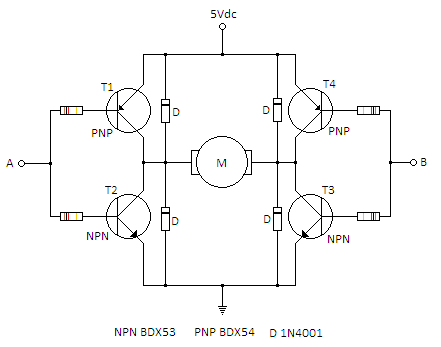
\includegraphics[scale=0.2]{schema.png}
    \caption{I valori errati dati dal reset automatico di thinkercad}
    \label{fig:logo}
\end{figure}
\vspace{.5\baselineskip}

    
    \vspace{1\baselineskip}
    \section{Cenni teorici e calcoli}
    Per prevedere l'evoluzione temporale del sistema si usa la formula:
    \begin{center}
        $Q_{(t)}=Q_{0}(1-e^{-t/\tau})$ \\
    \end{center}
    \noindent In questa formula si usa per determinare la carica in relazione del tempo, $Q_0$ rappresenta il livello massimo della carica. \\
    Mentre $\tau$ è una costante di tempo  data da $\tau=R*C$. 
    \\Questa costante di tempo serve a capire in quanto tempo il condensatore si carica, infatti $5\tau$ è uguale al tempo che serve al condensatore per essere carico al 95\% quindi il 95\% di $Q_0$ per effettuare un ciclo di carica e scarica completa il condensatore necessita di tempo uguale a $10\tau$ e di conseguenza compiere un periodo T. \\
    \begin{center}
        $\tau=R*C=1k\Omega*100nF=(1*10^3)*(100*10^{-9})=10^{-4}=0,1ms$\\
        \textit{f}$=1/T=1/10\tau=1/10^{-4}=10^4Hz=1kHz$\\
    \end{center}
    Il fatto che $5\tau$ siano il 95\% della carica massima non è un problema perché $Q_{(t)}$ non sarà mai uguale a $Q_0$ difatti si chiama \emph{asintoto}.\\
   
    \vspace{1\baselineskip}
    \section{Procedimento}
    Avendo calcolato la \textbf{frequenza massima} per far caricare completamente il condensatore possiamo montare il circuito collegando in serie la resistenza e il condensatore.\\ 
    Per vedere l'onda quadra del generatore si collega il puntale dell'oscilloscopio al reoforo della resistenza  collegato al generatore e il morsetto nero a massa, mentre per vedere il grafico del condensatore il puntale del secondo canale va collegato al reoforo del condensatore in serie con la resistenza e il secondo morsetto nero a massa.
    Dopo aver collegato tutto si procede a impostare il generatore per fargli generare un'onda quadra con tensione \textbf{picco picco} di \textbf{20V} e duty cycle al 50\% con frequenza che varierà seguendo la tabella.\\
    Una volta impostata la frequenza tramite il grafico si va a misurare quanto tempo dura un semi periodo, quanto vale la tensione che viene immagazzinata e rilasciata dal condensatore V\textit{f} e la differenza tra la tensione di picco e la V\textit{f} ossia $\Delta$V.
    
    \vspace{1\baselineskip}
    \section{Tabella}
    \begin{table}[H]
    \begin{tabular}{|c|c|c|c|c|c|} 
        \hline
        n° & \textit{f}[kHz] & Vmax[V] & \textit{T}/2 & V\textit{f}[V] & \Delta V \\ [0.5ex] 
        \hline
        1 & 0,5 & 20 & 1       & 10 & 0                         \\\hline
        2 & 1   & 20 & 0,5     & 10 & 0                         \\\hline
        3 & 2   & 20 & 0,250   & $\simeq$ 8,5 & $\simeq1,5$     \\\hline
        4 & 5   & 20 & 0,1     & 5   & 5          \\\hline
        5 & 7   & 20 & 0,074   & 3   & 7           \\[1ex] \hline
    \end{tabular}
    \label{tabella:es}
    \end{table}
        
    \vspace{1\baselineskip}
    \section{Conclusioni}
    Per le prime due misure le due onde sono quasi sovrapposte dal momento che la frequenza è abbastanza bassa per permettere al condensatore di  caricarsi completamente mentre aumentando la frequenza il condensatore si scarica prima di essersi caricato del tutto facendo diminuire V\textit{f} e aumentare $\Delta$V.\\
    Immagine dell'oscilloscopio con 0,5 kHz di frequenza:
    \begin{figure}[H]
    \centering
    \includegraphics[scale=0.1]{n1.jpg}
    \caption{Misura numero 1}
    \label{fig:n1}
\end{figure}

\noindent In questa immagine si può vedere appunto come il grafico del condensatore si avvicini a $Q_{0}$, mentre nelle immagini successive che rappresentano la misura numero 3 (2kHz) e 5 (7kHz) la curva si allontani sempre di più dal valore massimo.
   
\begin{figure}[h]
    \centering
    \begin{minipage}[b]{0.4\textwidth}
    \includegraphics[scale=0.1]{n3.jpg}
    \caption{Misura numero 3}
    \label{fig:n1}
    \end{minipage}
    \hfill
    \begin{minipage}[b]{0.4\textwidth}

    \centering
    \includegraphics[scale=0.1]{n5.jpg}
    \label{fig:n5}
    \caption{Misura numero 5}
    \end{minipage}
\end{figure}
\noindent Osservando le immagini si può notare che il condensatore si carica completamente quando $\textit{f}\leqslant1k$Hz
    
\end{document}
